\documentclass[a4j, titlepage]{jarticle}
\usepackage{url}
\usepackage{amsmath, amssymb}
\usepackage[dvipdfmx]{graphicx}

\title{基礎工学PBL 最終レポート}
\author{班名: 8班\\
担当教員: 松下 誠 准教授\\
氏名/学籍番号/電子メールアドレス:\\
岩越 唯人 09B23008 u618941g@ecs.osaka-u.ac.jp\\
梶村 優太 09B23019 u685627d@ecs.osaka-u.ac.jp\\
川原 歩夢 09B23021 u682459c@ecs.osaca-u.ac.jp\\
清原 佑介 09B23026 u643925a@ecs.osaka-u.ac.jp\\
坂井 峻大 09B23033 u681747f@ecs.osaka-u.ac.jp\\
林 宏祐 09B23065 u653793g@ecs.osaka-u.ac.jp
}
\date{提出日:\today}

\begin{document}
\maketitle

\section{課題1,2の概要}
私たち8班は,「高校教員の長時間労働問題と,これに付随する進路指導の質の低下」という社会問題について調査を行った.

この問題の背景として,教員は進路指導を行う義務を負うと法的に定められていること,また教員が生徒を様々な側面において支援するという実務的な問題などが存在している.その結果,高校教員の労働時間が増大する中で進路指導を行わなければならず,進路選択のミスマッチを誘発し得る,進路指導の質の低下が観測されている.また,別の側面では,教職員が長時間労働を強いられていることが,教職員における休職者数や自殺者数の増加に寄与していることも問題視されている.

これに対し,民間・行政ともに様々な対策を練っている.キャリア教育プログラム,職業体験,といった,情報科学技術を強く必要としないものから,求人票のデータ化を支援するサービスや,試験の点数や興味を持っている分野などのデータを蓄積できるシステムなど,情報科学技術を活用したものまで存在する.

以上のことを踏まえ,私たちは,あまり一般的ではない,「生徒が様々な質問に回答することで,希望に沿った大学群が提示される,日常的に利用できるサービス」の開発を目指すことにした.

具体的な方法を説明する.まず,大学の学部・学科,専攻,といったデータを集め,それを1つのデータベースに集約させる.ここに,生徒自身のデータ,例えば定期試験の点数,内申点,希望する専攻分野などを追加する.その上で,生徒にウェブ上で進路決定に関するいくつかの質問に答えてもらう,その結果と生徒の情報を比較して,生徒一人一人に適した条件を持つ,またはその条件に近い大学を提示する.

私たちは,このサービスの開発・普及により,生徒には進路に関する選択肢の適正化や幅の広さを知ってもらうきっかけに,教職員には進路指導に割く時間の削減につながる糸口になることを期待している.しかし,サービス実装に対する残された時間を考慮して,私たちは「生徒に進路の選択肢を提供するシステムのアルゴリズムを考案し,それを実装する」ことを目的と定めた.

\section{採用したソフトウェア,採用した理由}

\section{メンバー間での作業分担方針,実際の作業分担結果}

\subsection{作業分担方針}
\begin{itemize}
\item フロントエンド : 岩越唯人,坂井峻大,林宏祐
\item バックエンド : 梶村優太,清原佑介
\item API通信・全体のサポート : 川原歩夢
\end{itemize}

\subsection{実際の作業分担結果}
\begin{itemize}
\item{フロントエンド} \\
質問やバックエンドから受け取った大学の一覧を画面に表示するプログラムを組むことができた.また,画面表示のデザインを全体的に統一し,UI/UXの向上に努めた.
\item{バックエンド} \\
データベースから取得した大学のデータをモックし,その中から質問の回答に合致する大学を抽出するプログラムを組むことができた.
\end{itemize}

\section{動作環境}
動作環境には,Node.js:20.15.0,Google Chrome(v8)を採用した.
\section{環境構築手順}

\section{動作結果}
ここでは実際にシステムを動作させたときの様子を示していく.

\begin{figure}[h]
  \centering
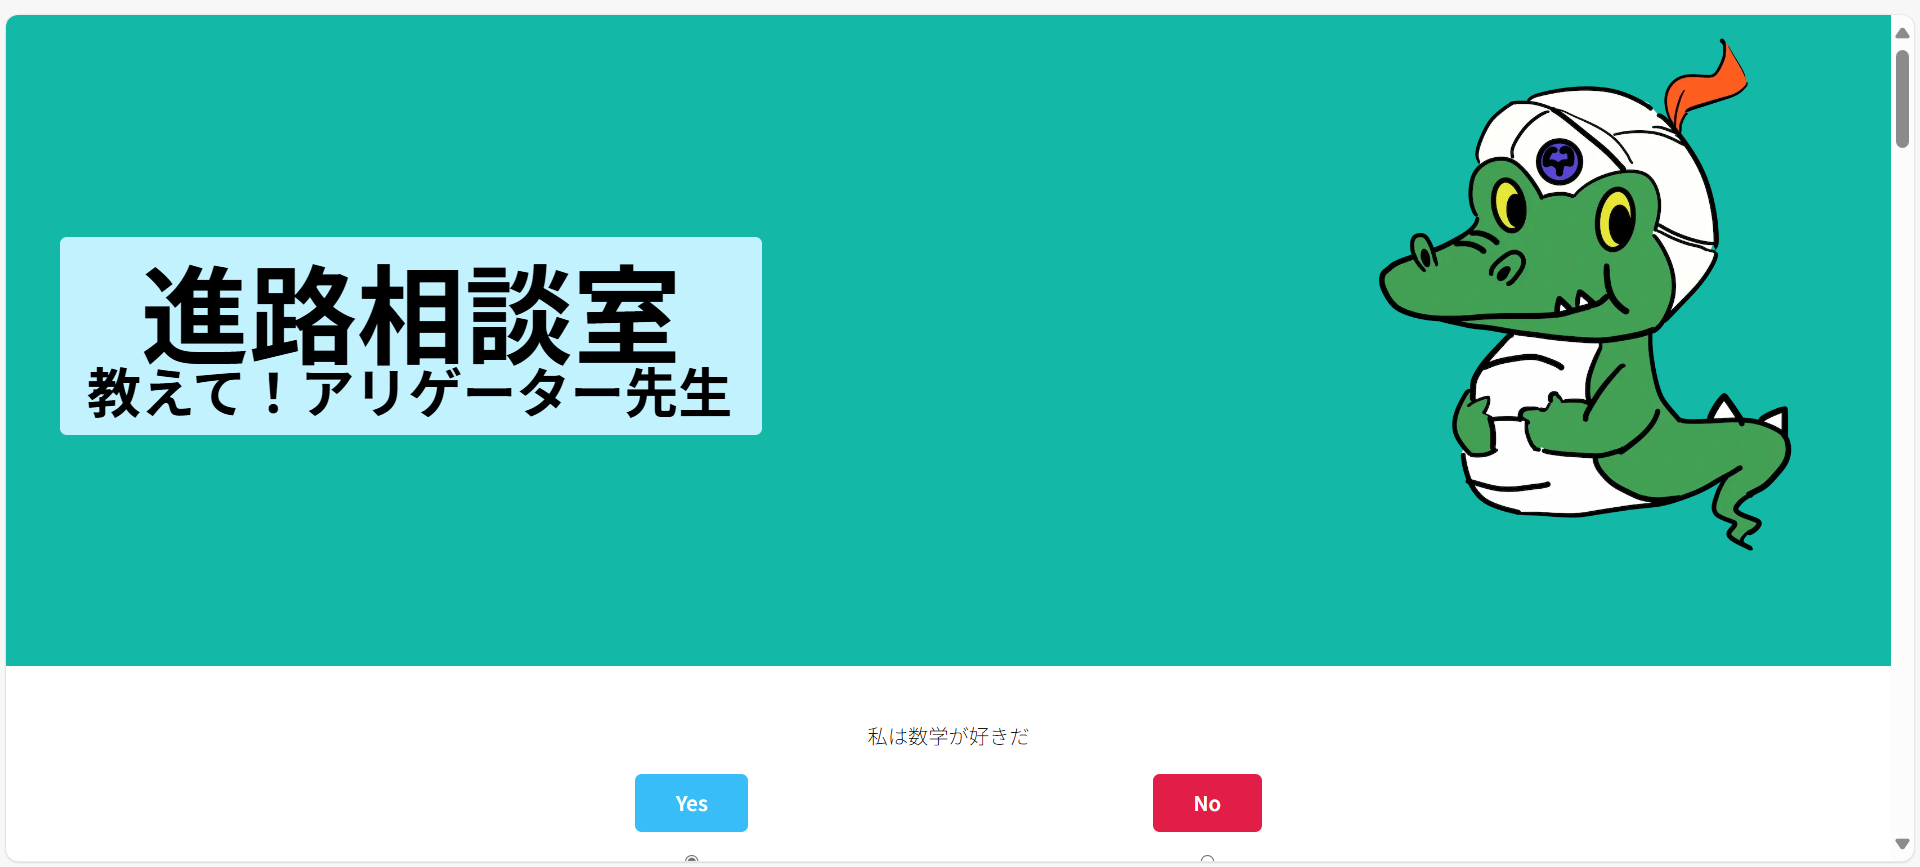
\includegraphics[scale=0.20]{dousakekka-1.png}
\caption{ウェブ起動時}
\end{figure}

スクロールしながら質問に答えていく.

\begin{figure}[h]
  \centering
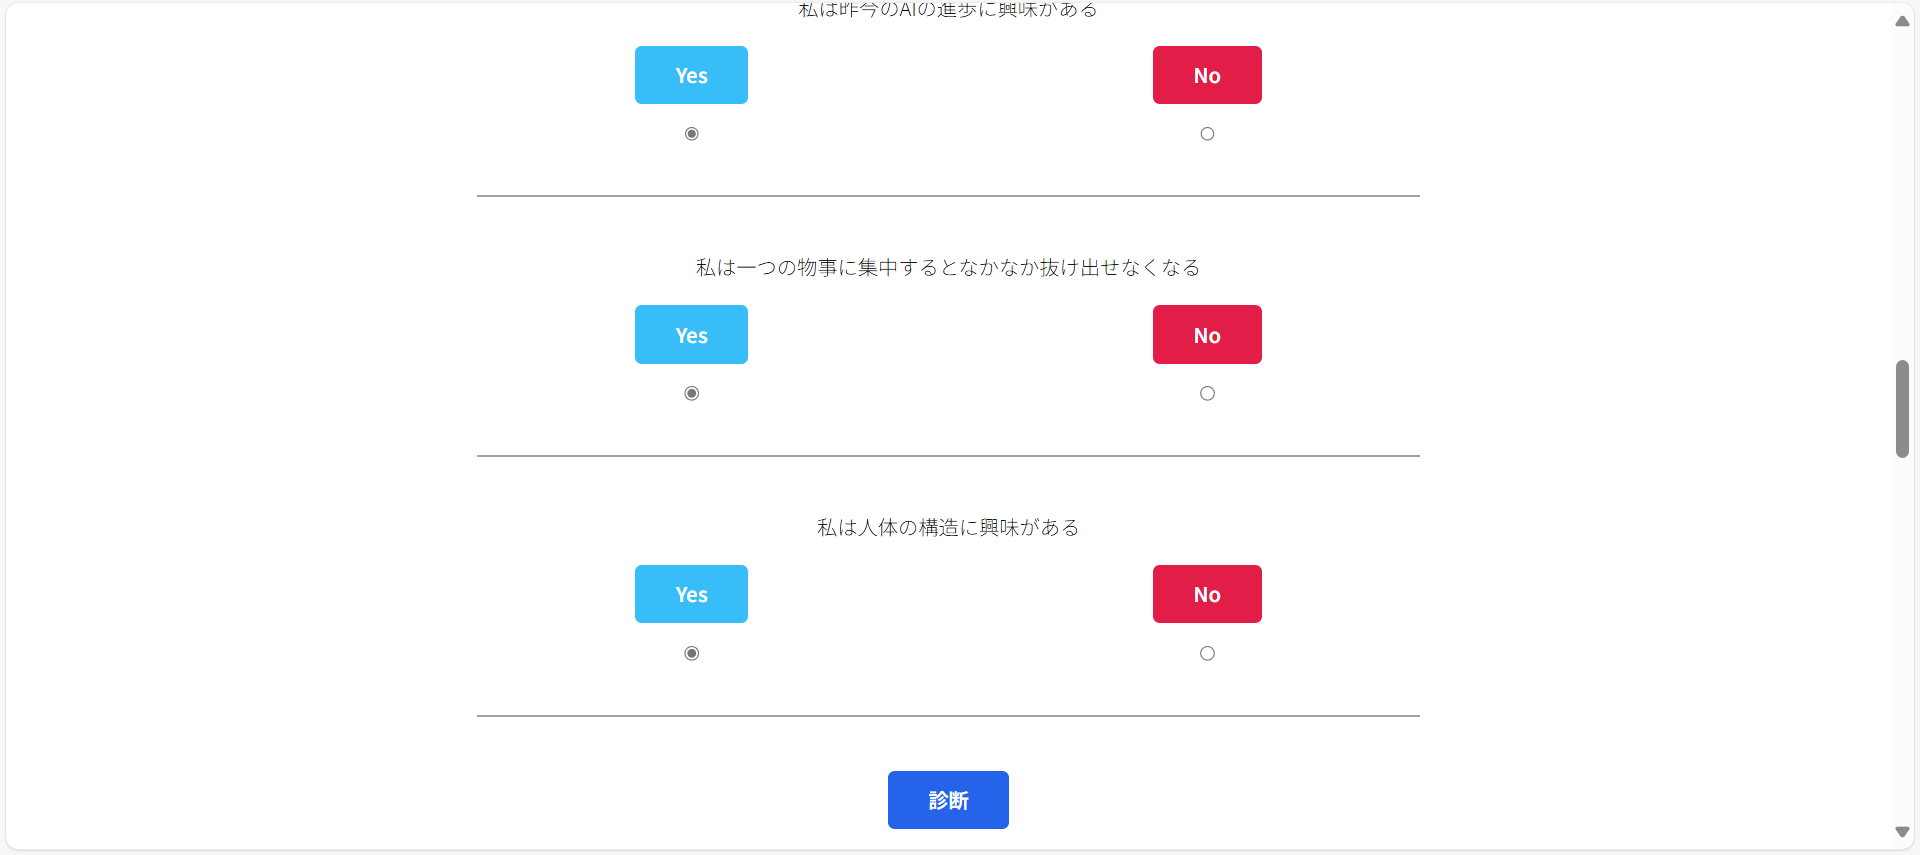
\includegraphics[scale=0.20]{dousakekka-2.png}
\caption{質問解答}
\end{figure}

質問への解答はYes or No.
各々の質問に解答した後,診断ボタンを押すことで該当する大学名を表示.

\begin{figure}[h]
  \centering
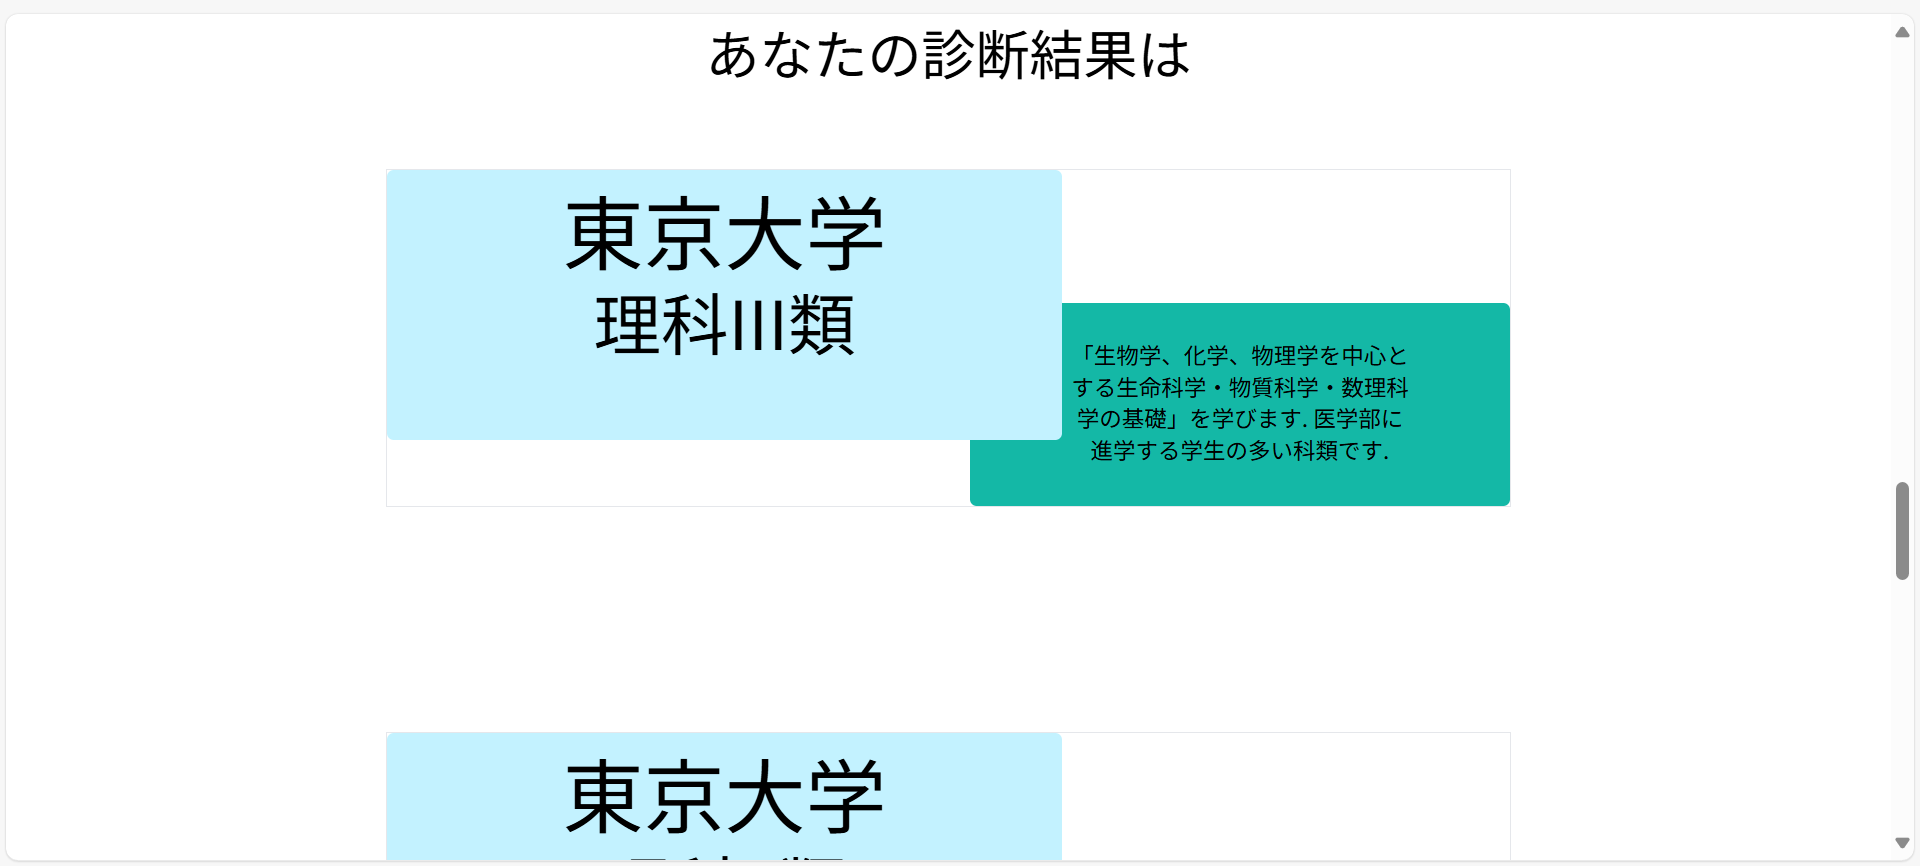
\includegraphics[scale=0.20]{dousakekka-3.png}
\caption{診断結果の表示}
\end{figure}

該当大学,学部とその簡単な説明を表示する.
該当する大学が複数個存在する場合,それぞれ表示する.

以下に,異なる解答をした場合の診断結果について表示する.

一般的に理系的であると捉えられる解答をした場合.

\begin{figure}[h]
  \centering
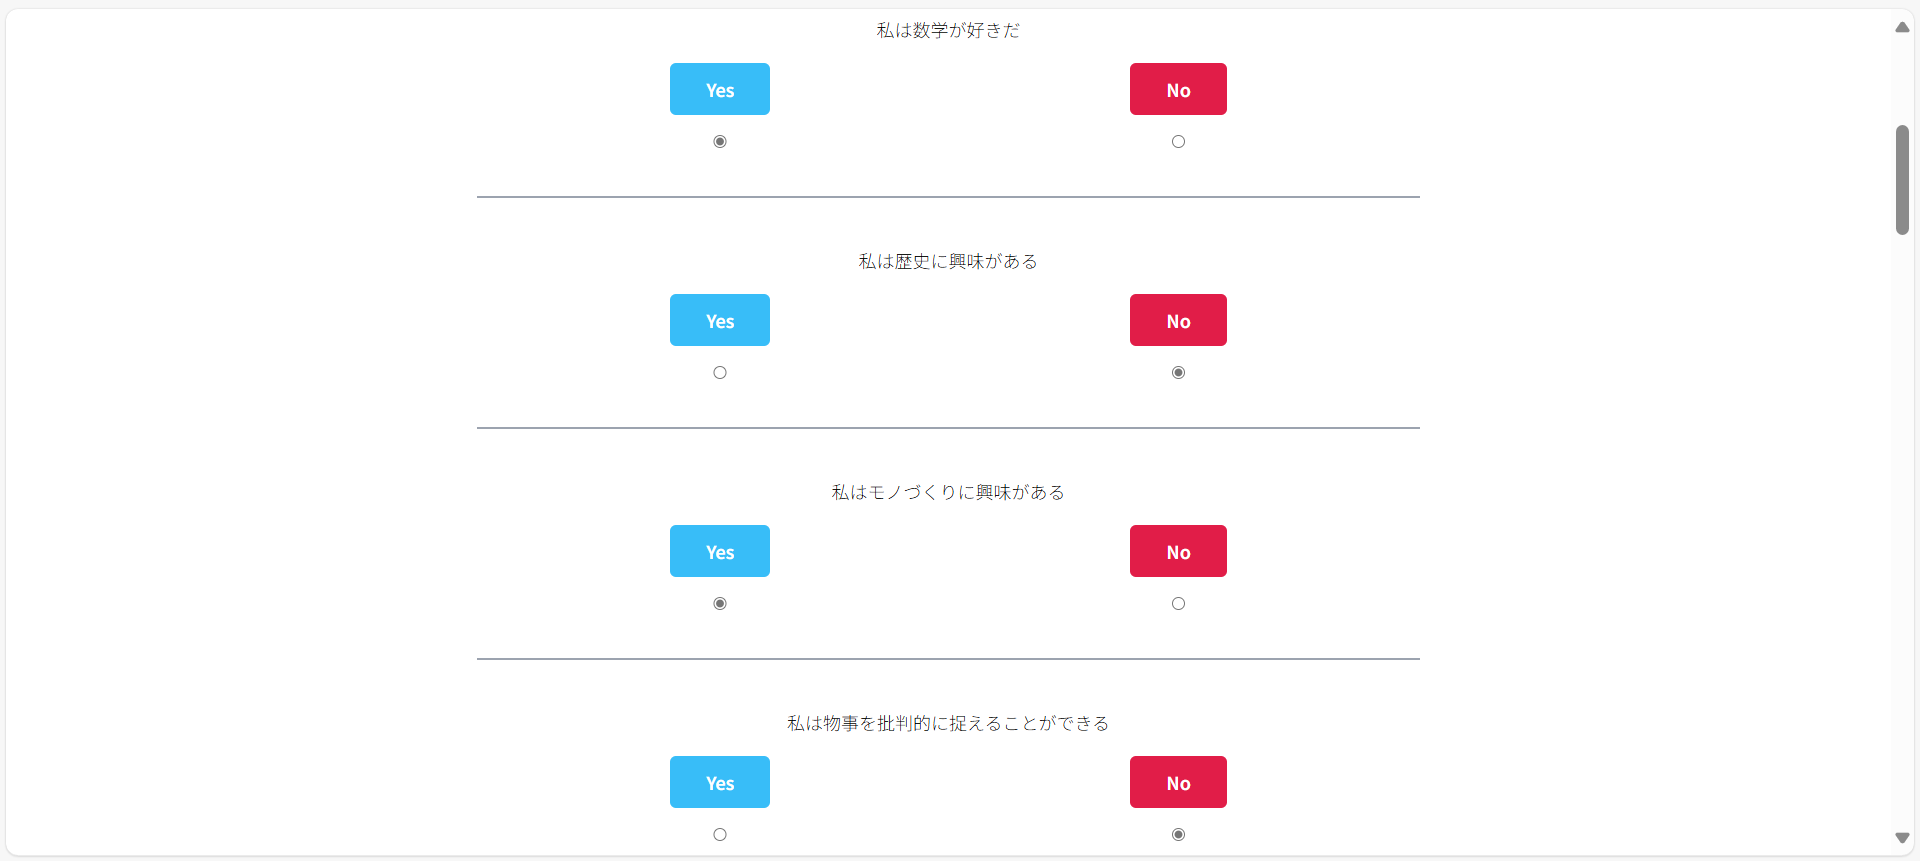
\includegraphics[scale=0.20]{dousakekka-4.png}
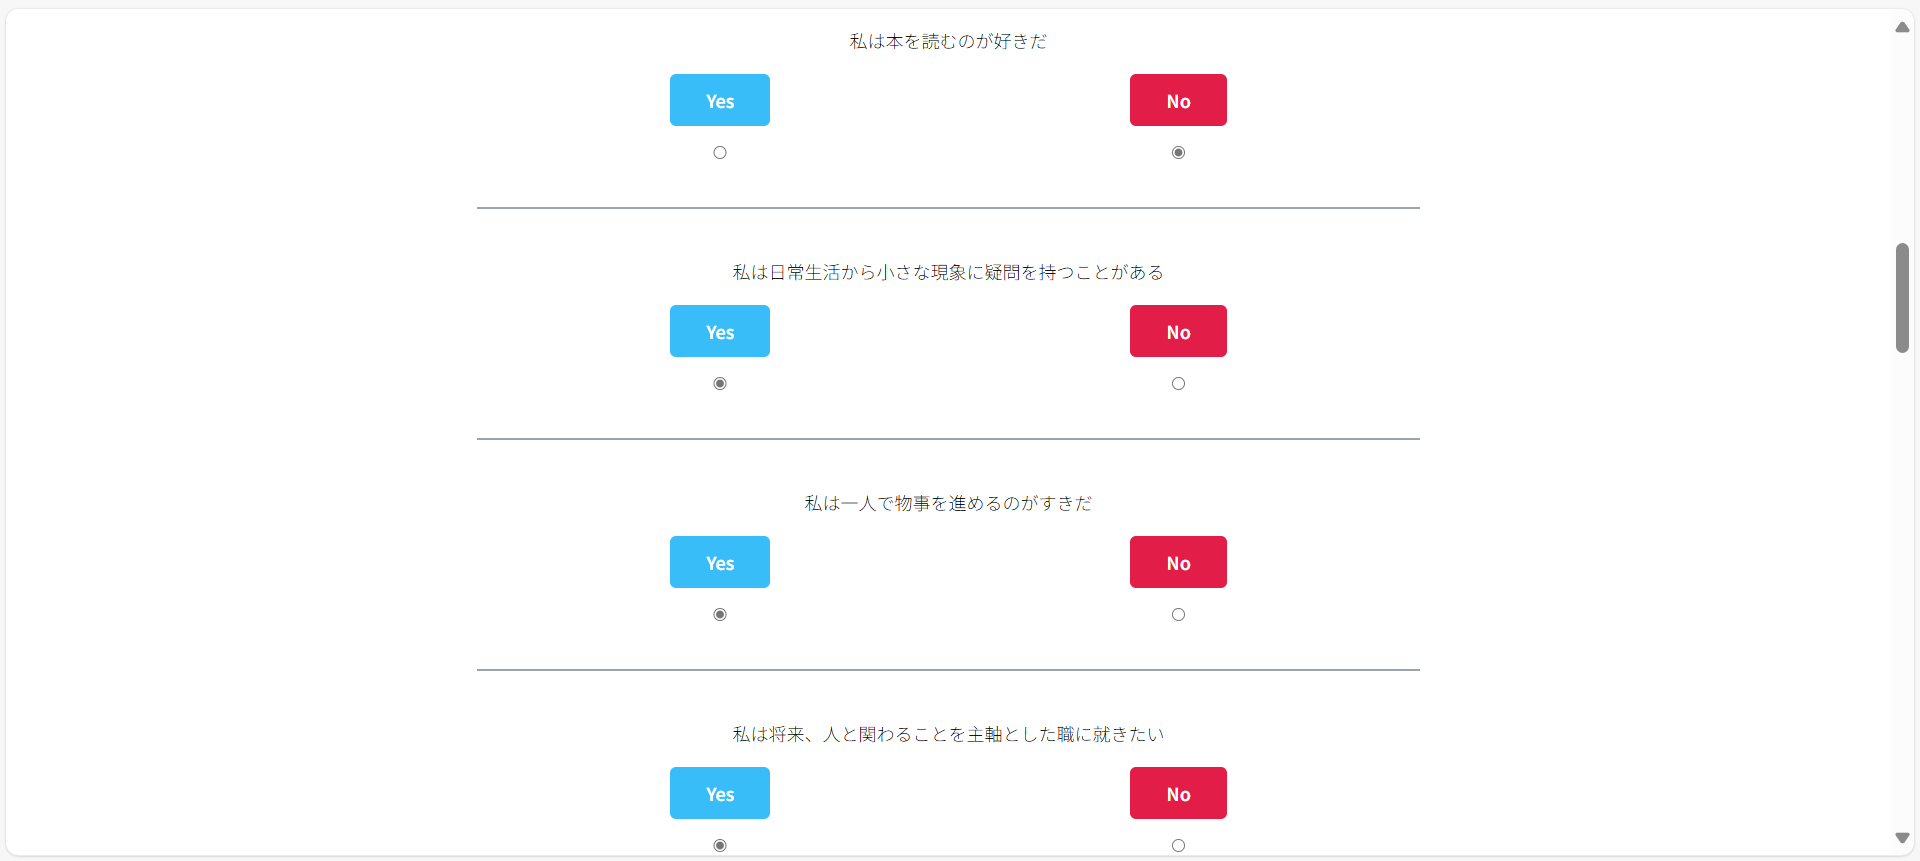
\includegraphics[scale=0.20]{dousakekka-5.png}
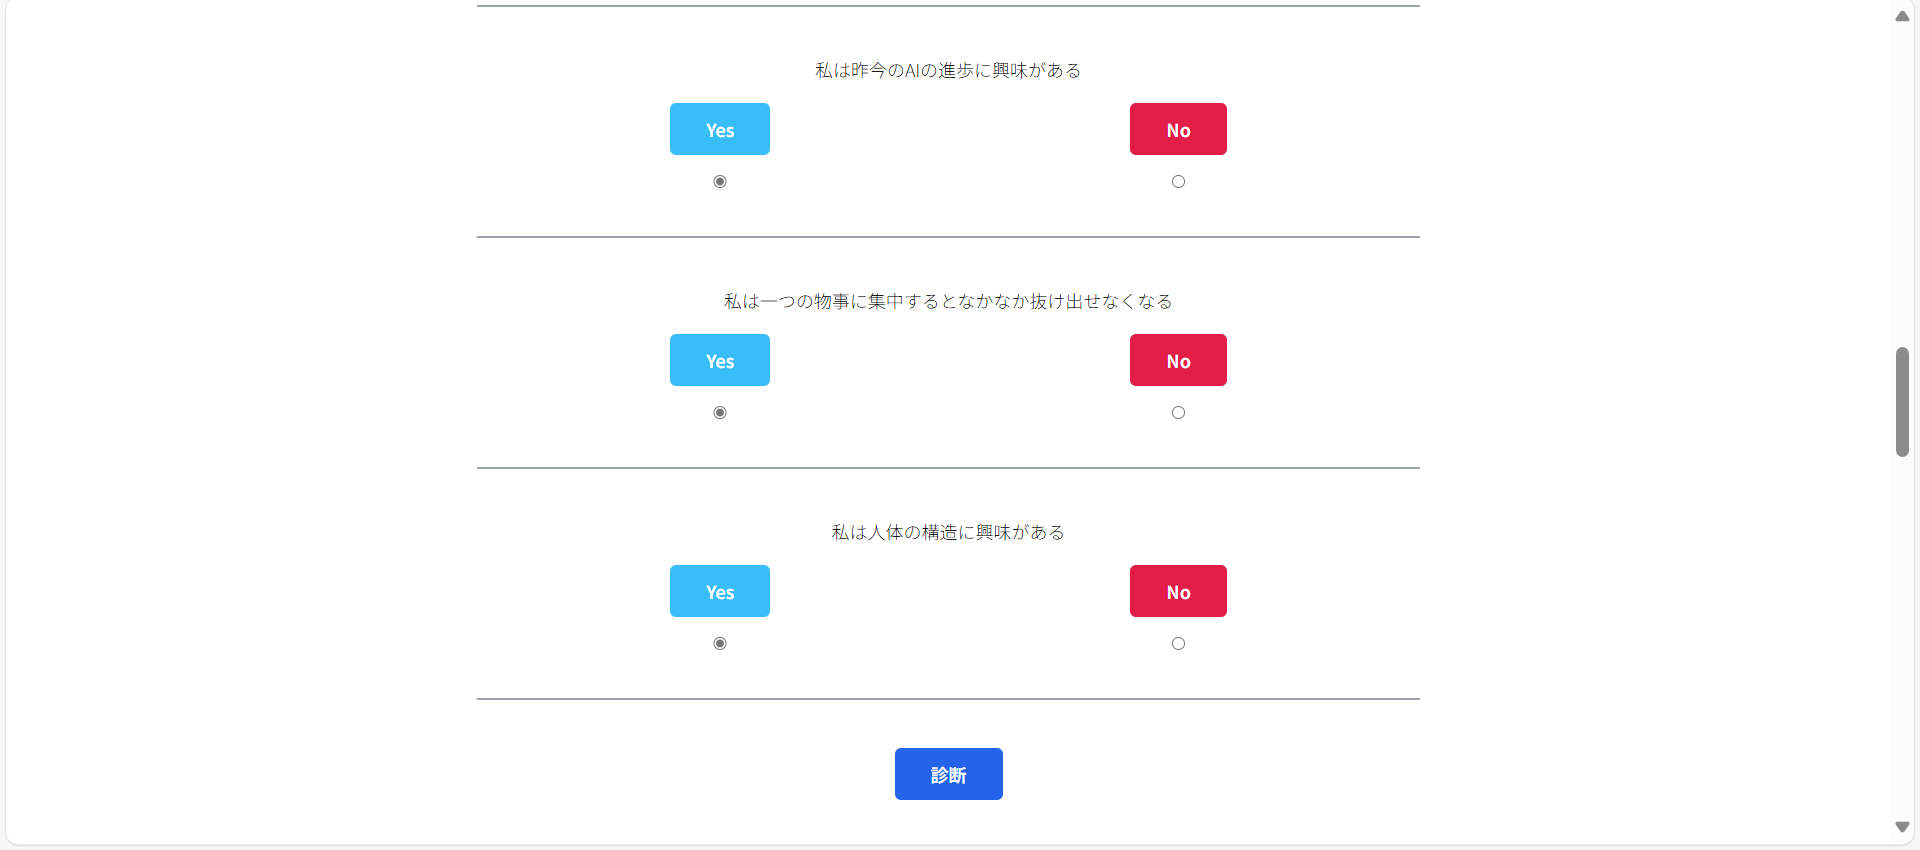
\includegraphics[scale=0.20]{dousakekka-6.png}
\end{figure}

その結果.

\begin{figure}[h]
  \centering
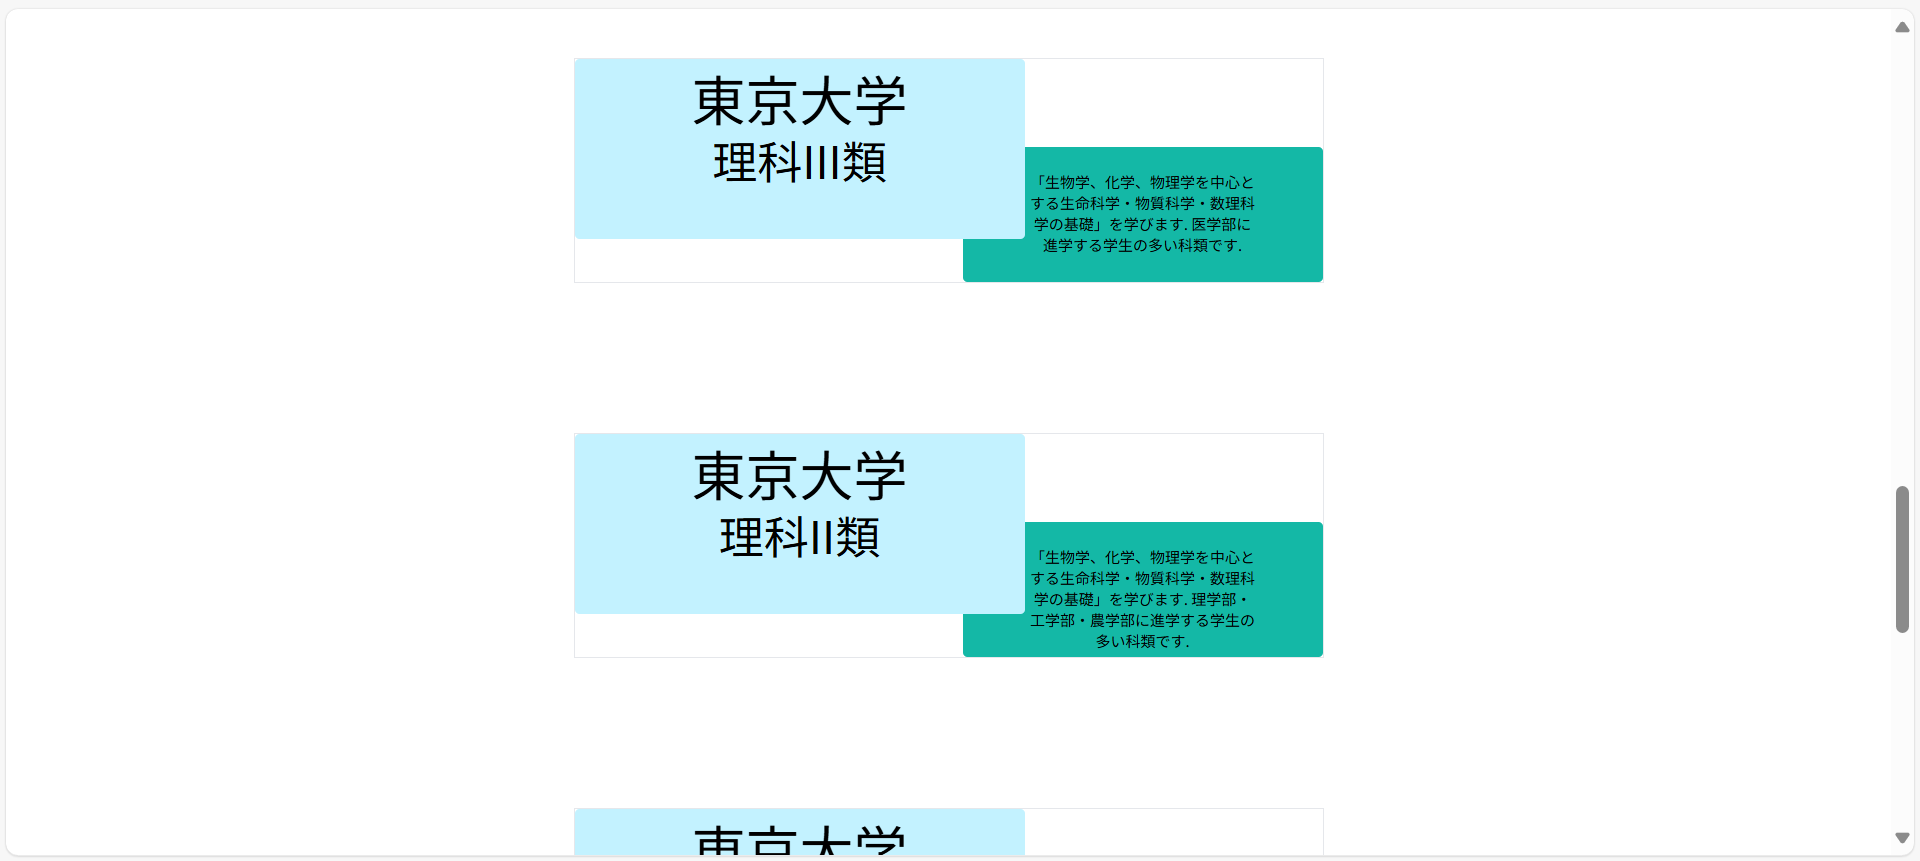
\includegraphics[scale=0.20]{dousakekka-7.png}
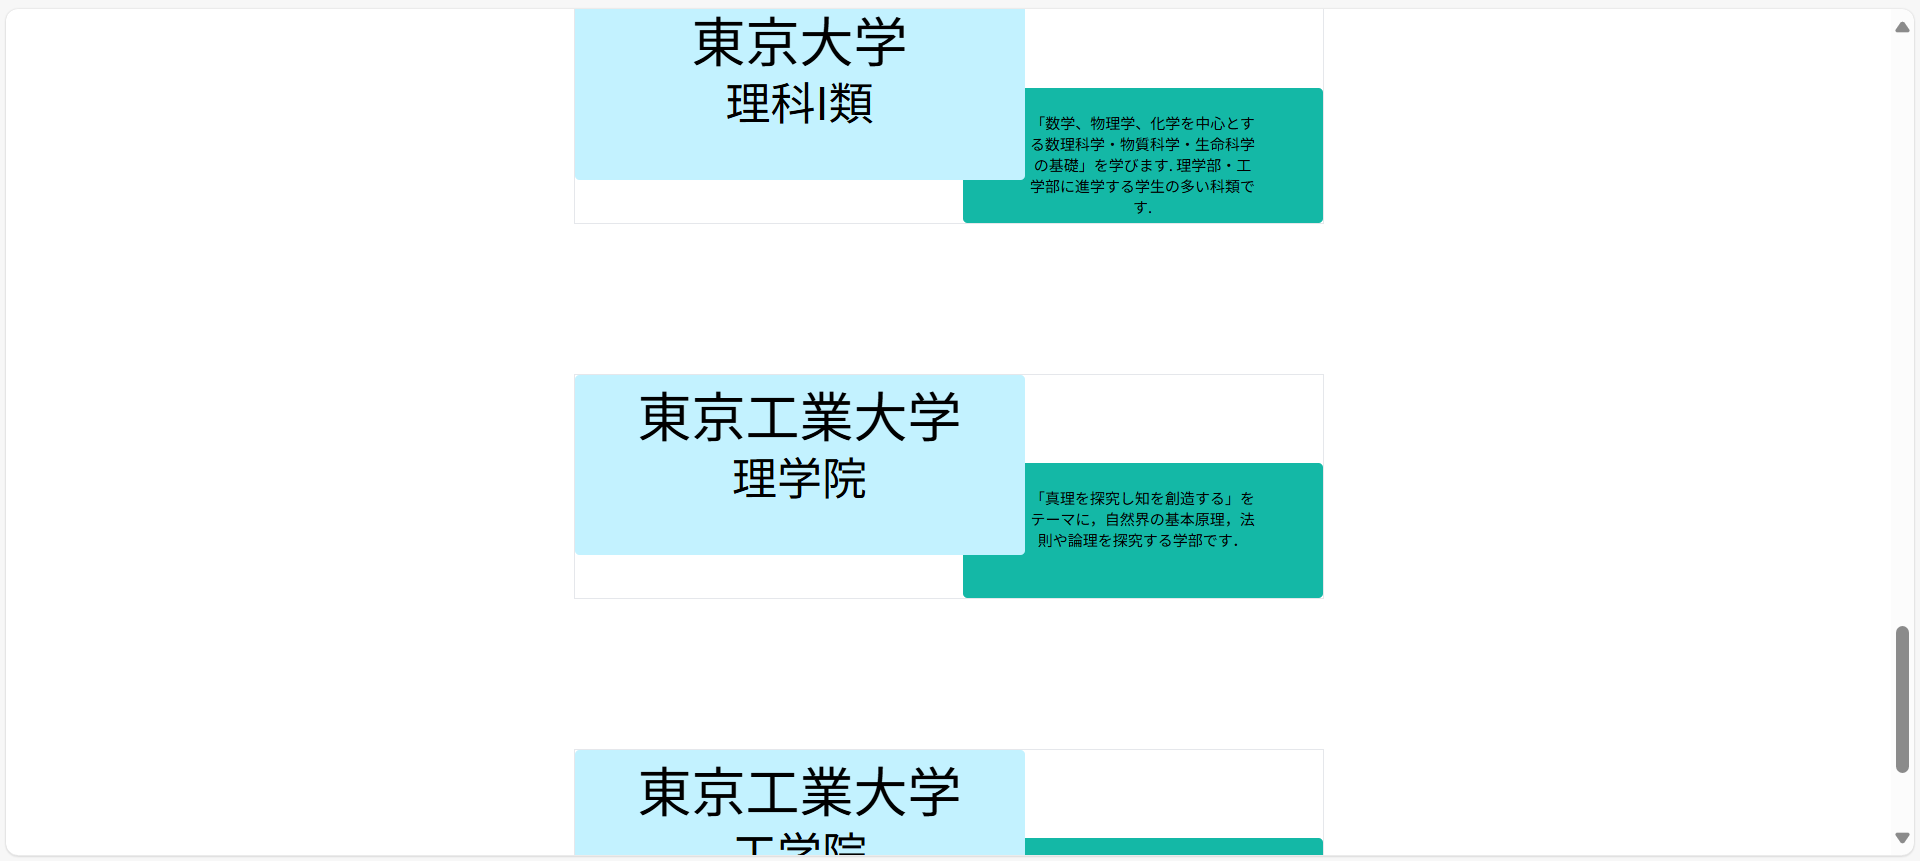
\includegraphics[scale=0.20]{dousakekka-8.png}
\end{figure}

理系の大学学部が表示されている.

一般的に文系的であると捉えられる解答をした場合.

\begin{figure}[h]
  \centering
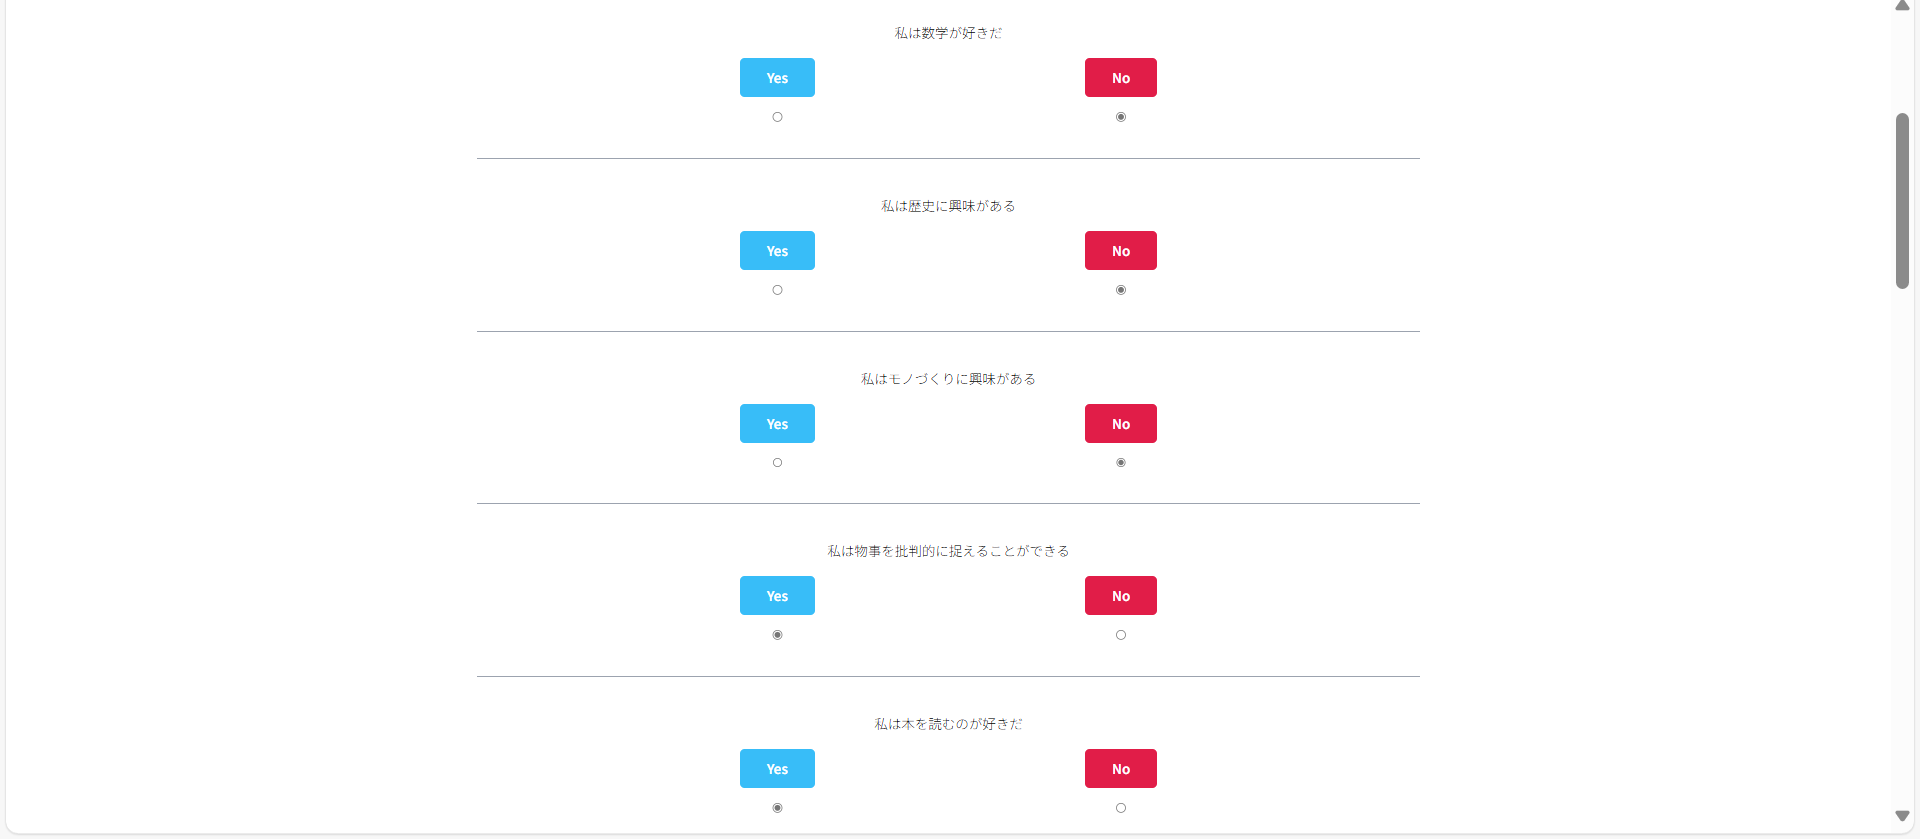
\includegraphics[scale=0.20]{dousakekka-9.png}
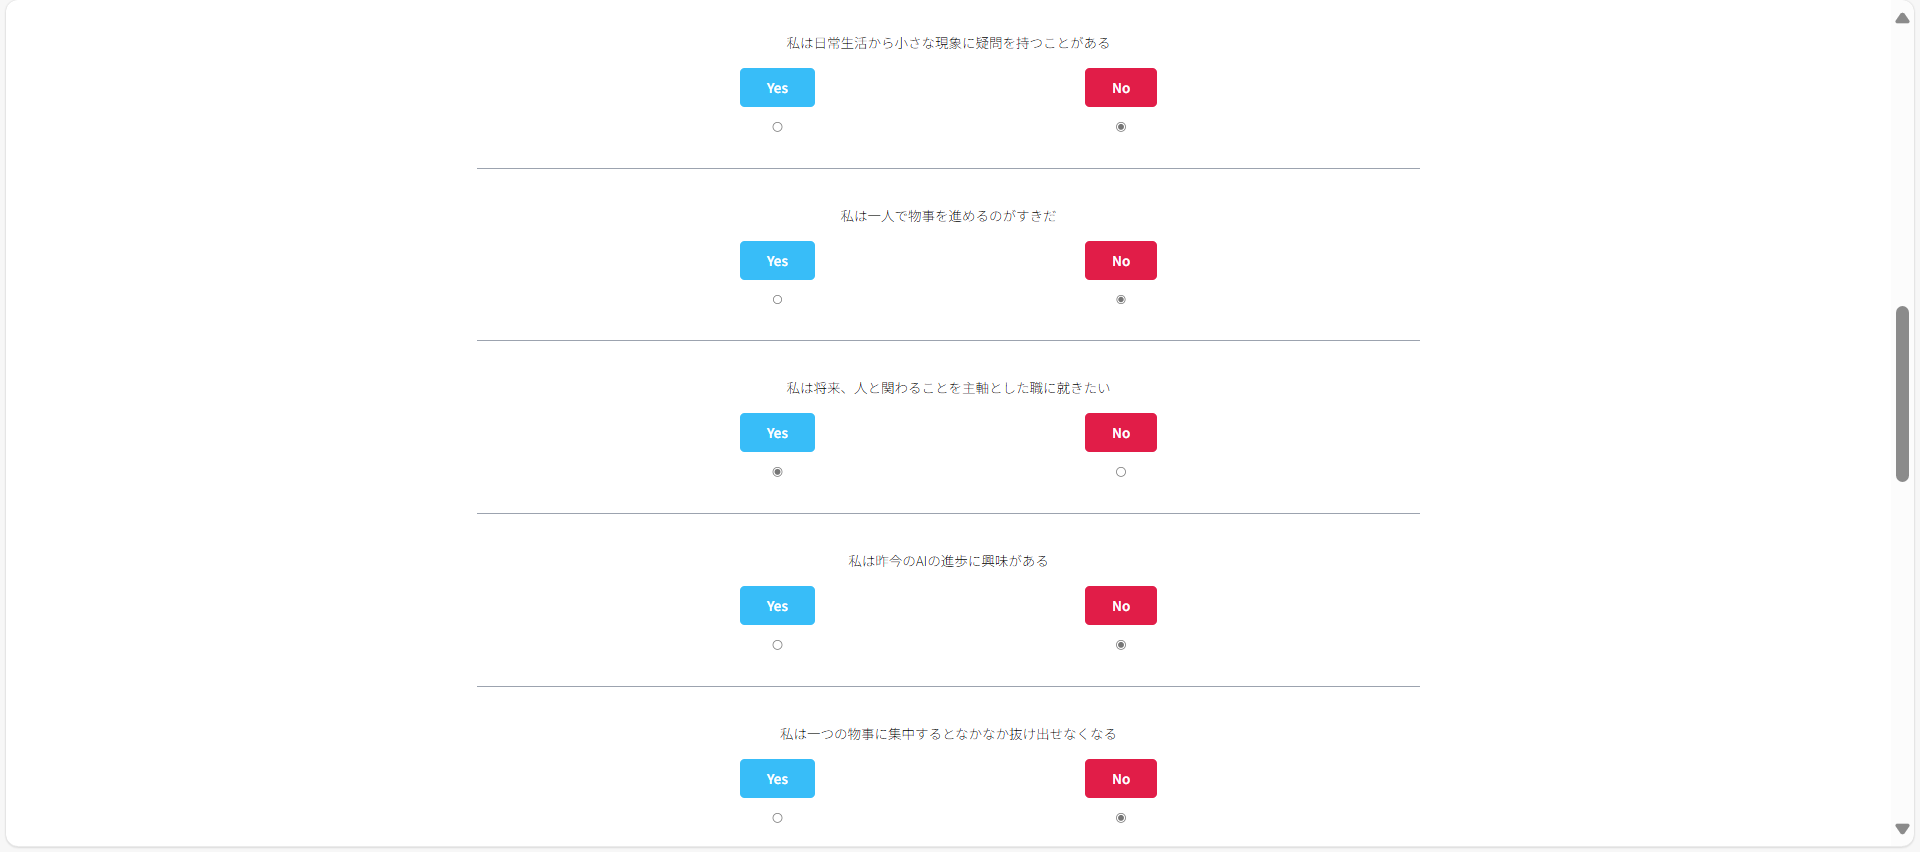
\includegraphics[scale=0.20]{dousakekka-10.png}
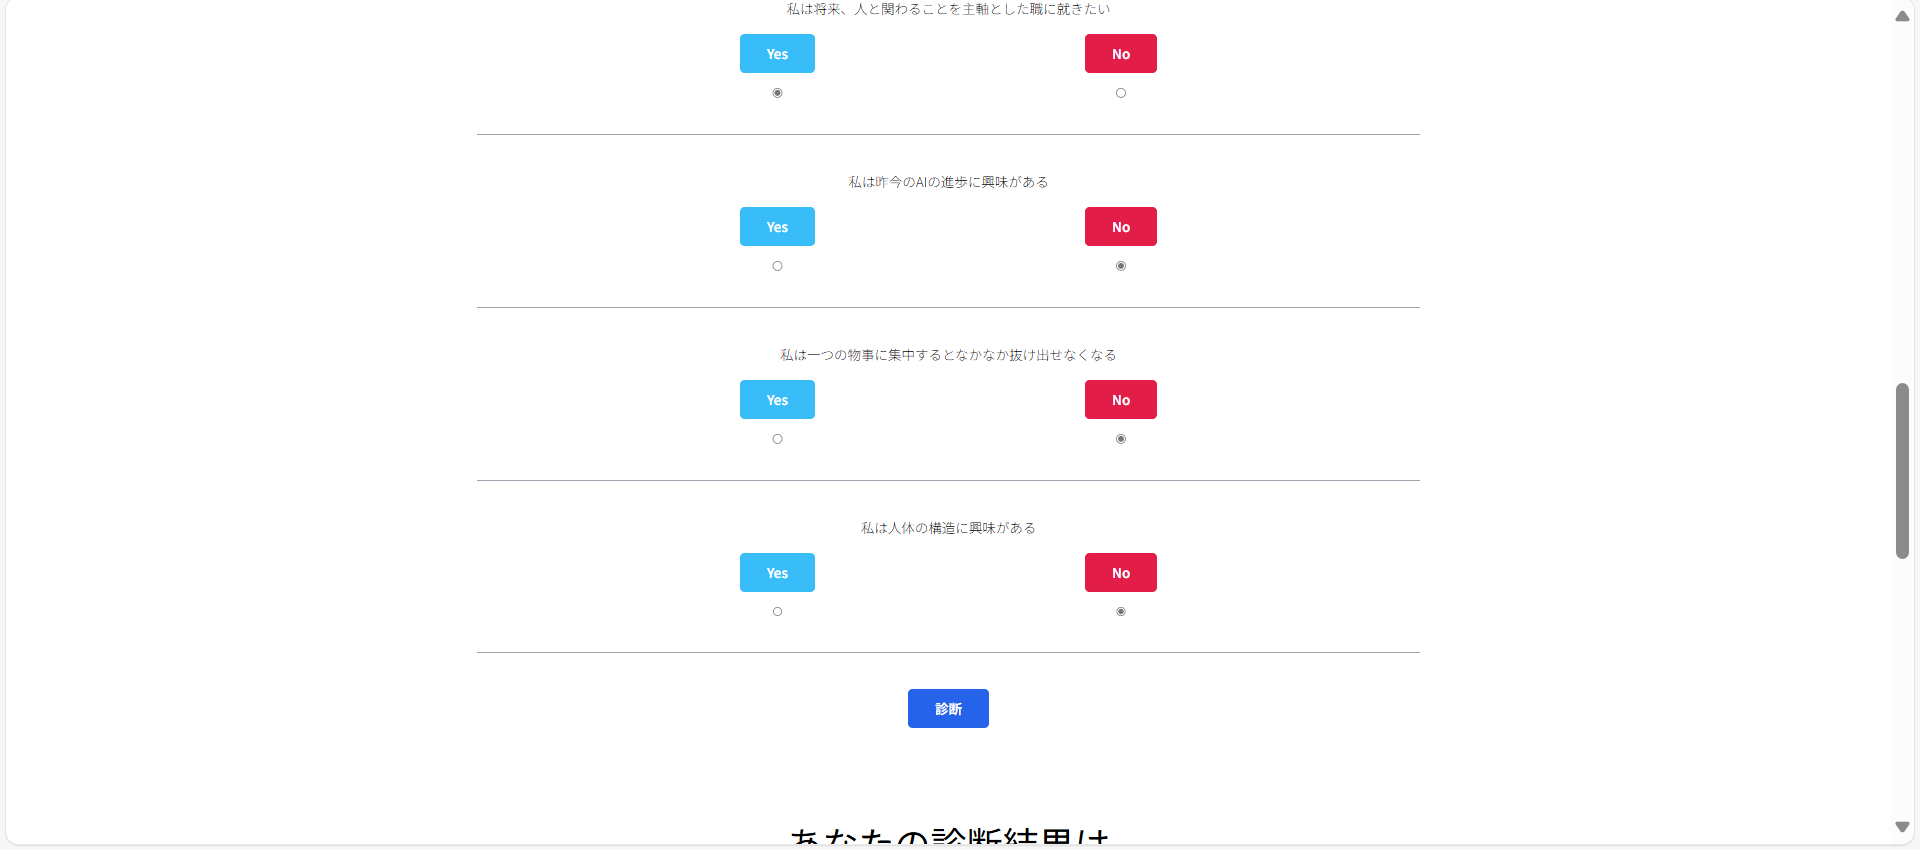
\includegraphics[scale=0.20]{dousakekka-11.png}
\end{figure}

その結果.

\begin{figure}[h]
  \centering
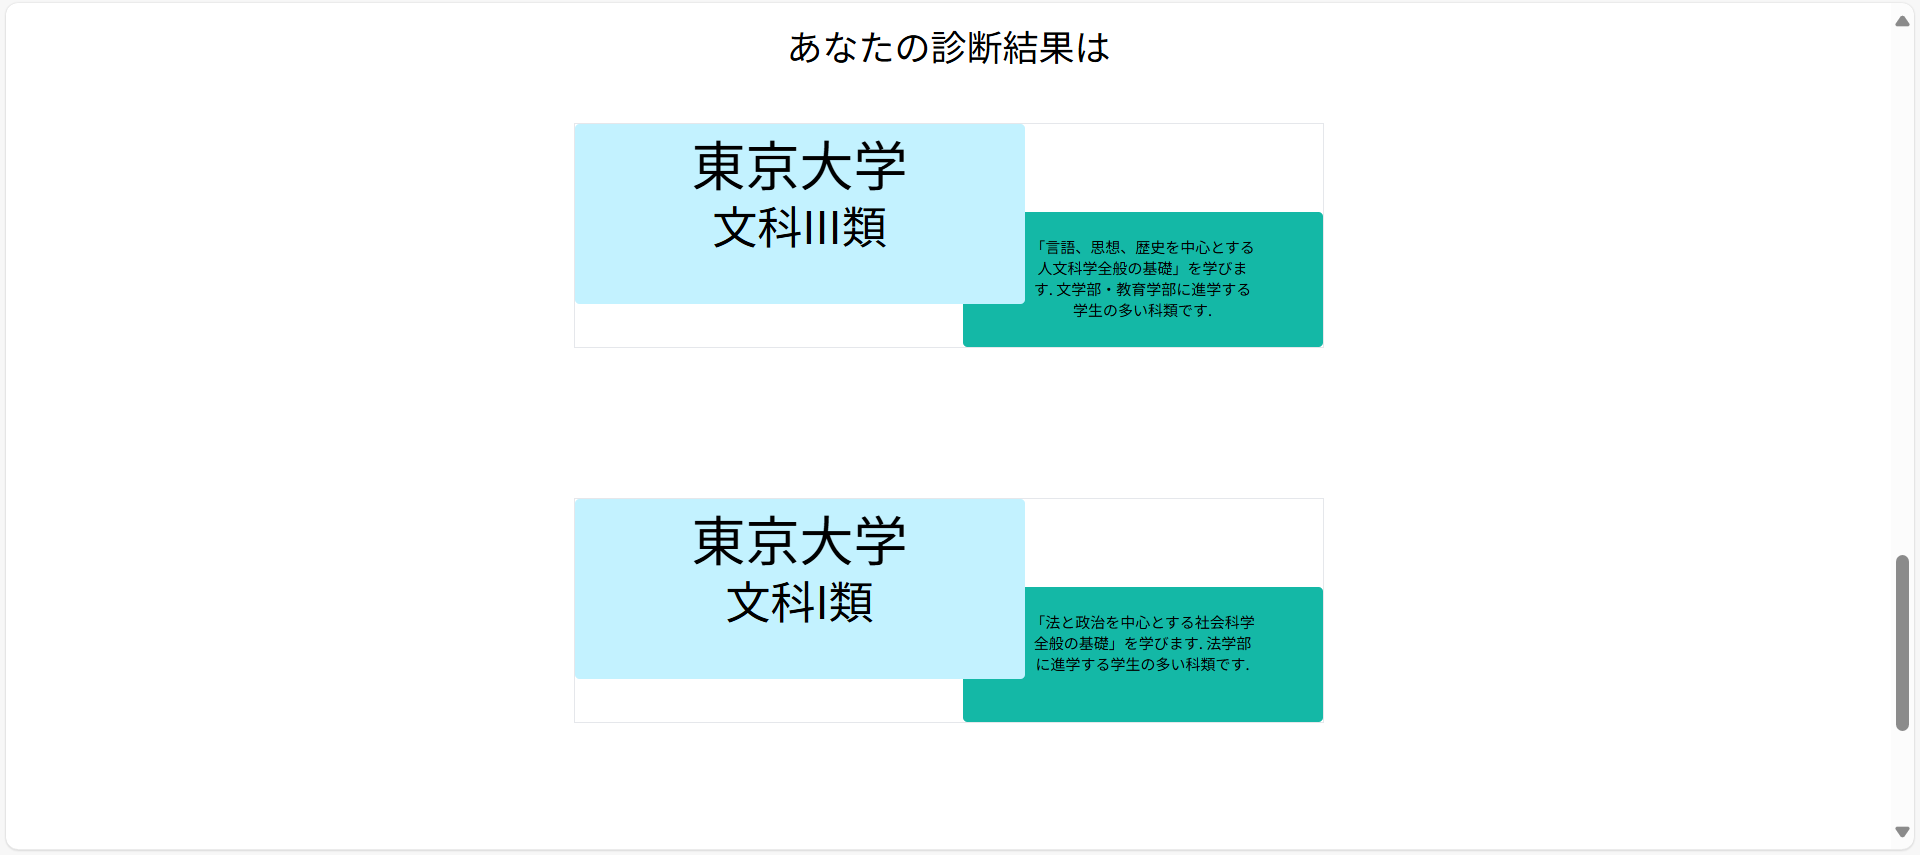
\includegraphics[scale=0.20]{dousakekka-12.png}
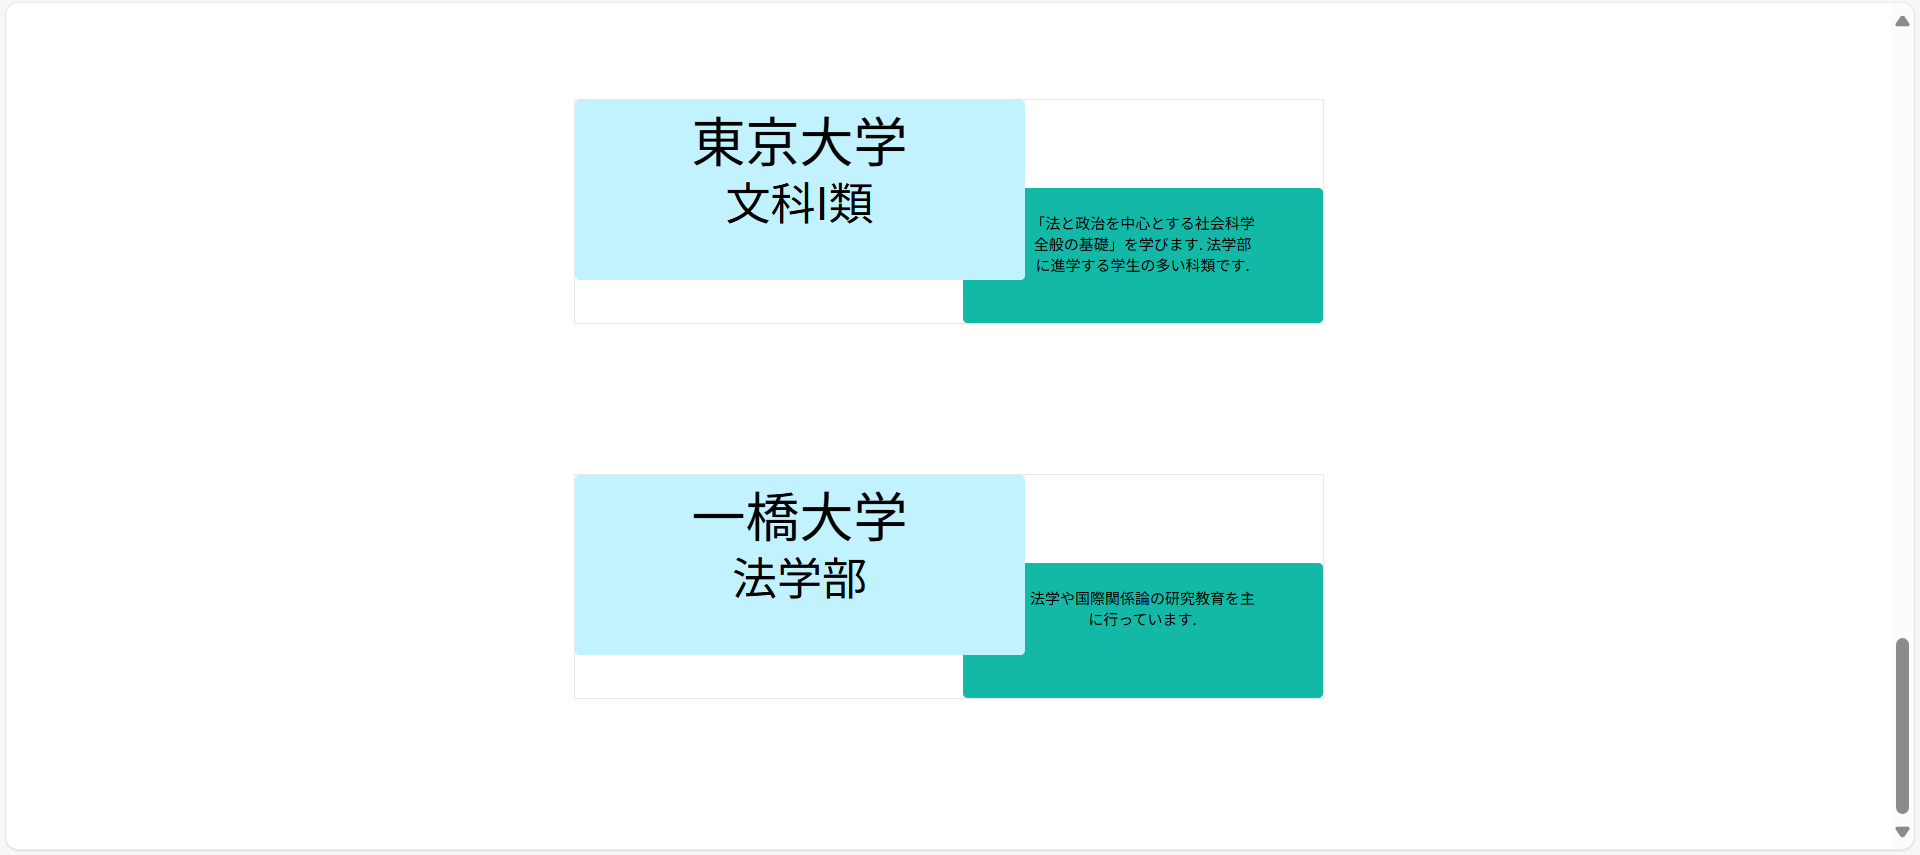
\includegraphics[scale=0.20]{dousakekka-13.png}
\end{figure}

文系の大学学部が表示されている.

\section{課題3で最も苦労した点,次に苦労した点}
\subsection{最も苦労した点}

私たちが課題3で最も苦労した点として,githubを用いた共同開発があげられる.
課題1,2を通して進路選択を支援するwebアプリケーション制作を決定した私たちは,githubを用いて共同開発をすることにした.
しかし私たちはメンバーのほとんどが共同開発の経験がなく,したがってまずgithubのアカウントを作り,その使い方を学習することから始めた.

アカウントを作った後,まず最初にcommit,push,pullの方法を学んだ.
この時点ではgithubがどういったものかも理解していなかったので,commit,push,pullの方法に交えてgithubの基本的な考え方についても学んだ.

次に,branch,pullrequest,mergeについて学んだ.
この時点で,最低限の知識はついたと判断し,webアプリケーションの制作を開始した.

最後に,conflictについて学んだ.
conflictについては,実際にconflictが起きたときに,それを解消していくという手順で学んだ.
特にconflictについては,作業分担をしているとはいえ,同じファイルを同時進行で編集する場面も多々あったので苦労した.

しかしこれらの苦労を乗り越えた結果として,githubを用いた集団での開発方法をメンバー全員が身に着け,進路選択支援のwebアプリケーションを制作することができた.
\subsection{次に苦労した点}
私たちが課題3で次に苦労した点として,進路選択を支援するwebアプリケーションのUIデザインがあげられる.
私たちはメンバー全員がwebサイトのデザインについての知識がなかったため,UIについては試行錯誤を繰り返しながらの制作となった.
つまり,構想したデザインを実際に作ってみてはそれについて評価を下し,改善を繰り返すという形式となった.

見やすさ,使いやすさ,そして見た目の良さにも気を向けたUIの制作は簡単ではなかったが,最終的にメンバー全員が納得する出来のUIを制作することができた.
特に,デザイン担当が自ら描いてくれたタイトル画面のアリゲーター先生には,私たちの作ったwebアプリケーションのコンセプトを一目で理解させる効果を期待している.\\


以下は,最終的なタイトル,フォーム,希望に沿った大学群のデザインである.
\begin{figure}[htbp]
  \begin{center}
  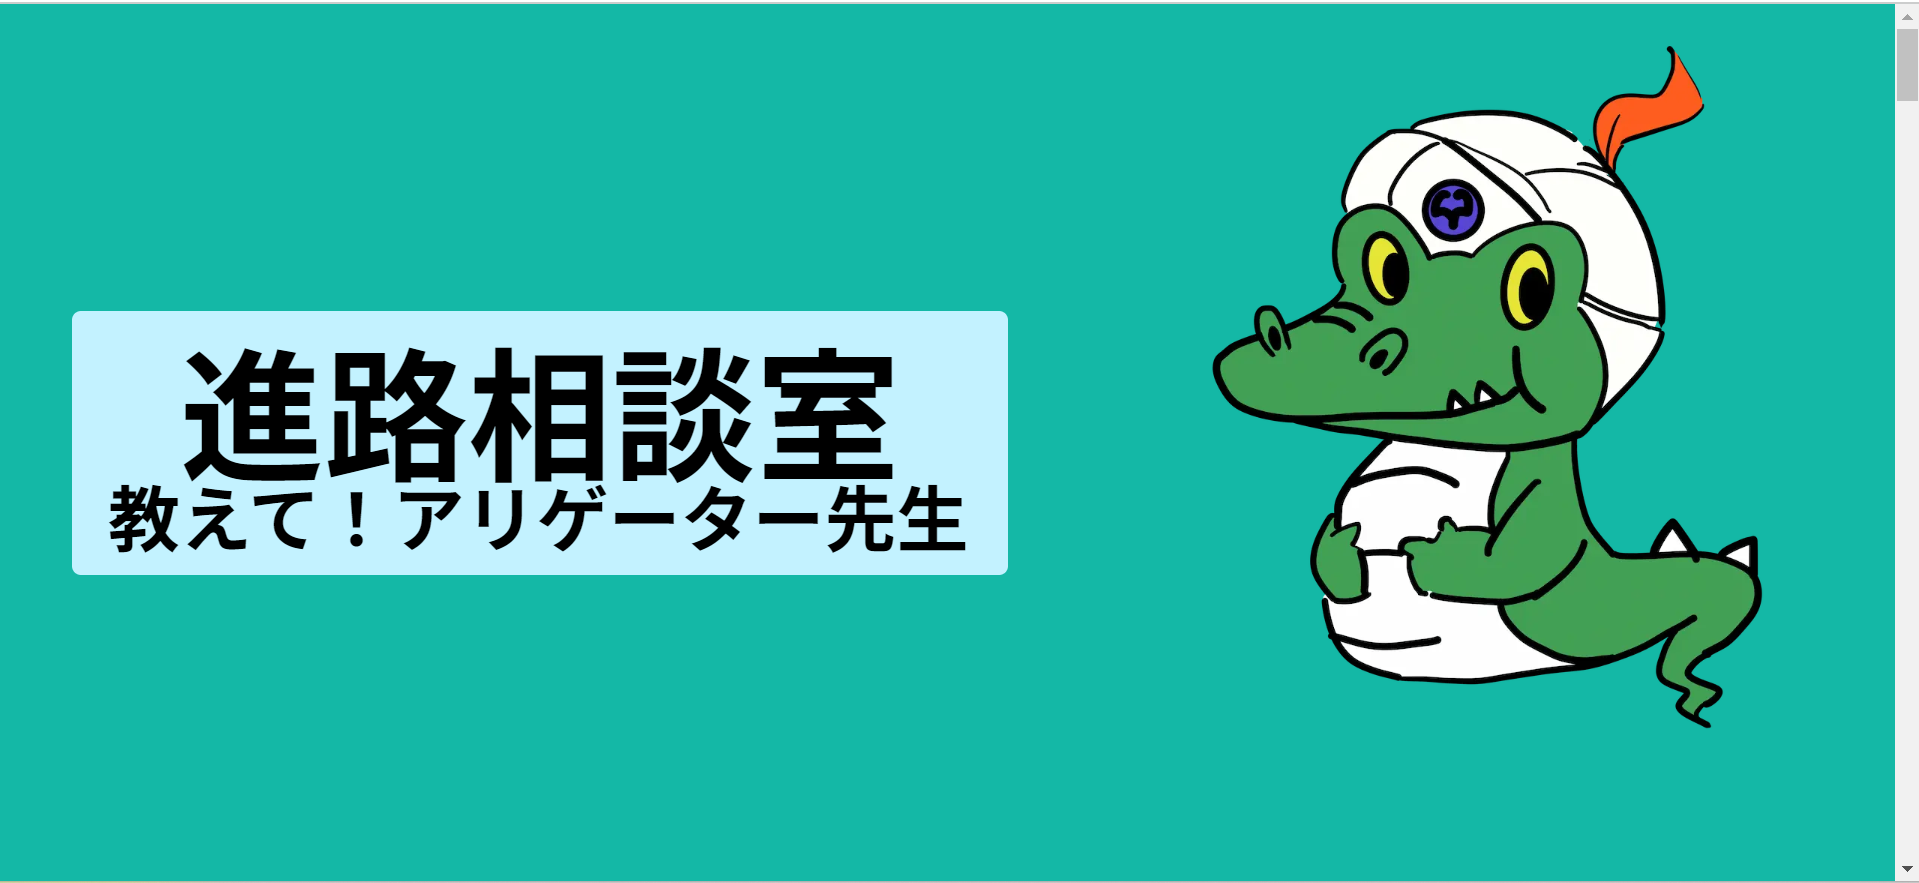
\includegraphics[width=100mm]{title.png}
  \caption{タイトル}
  \end{center}
\end{figure}
\begin{figure}[htbp]
  \begin{center}
  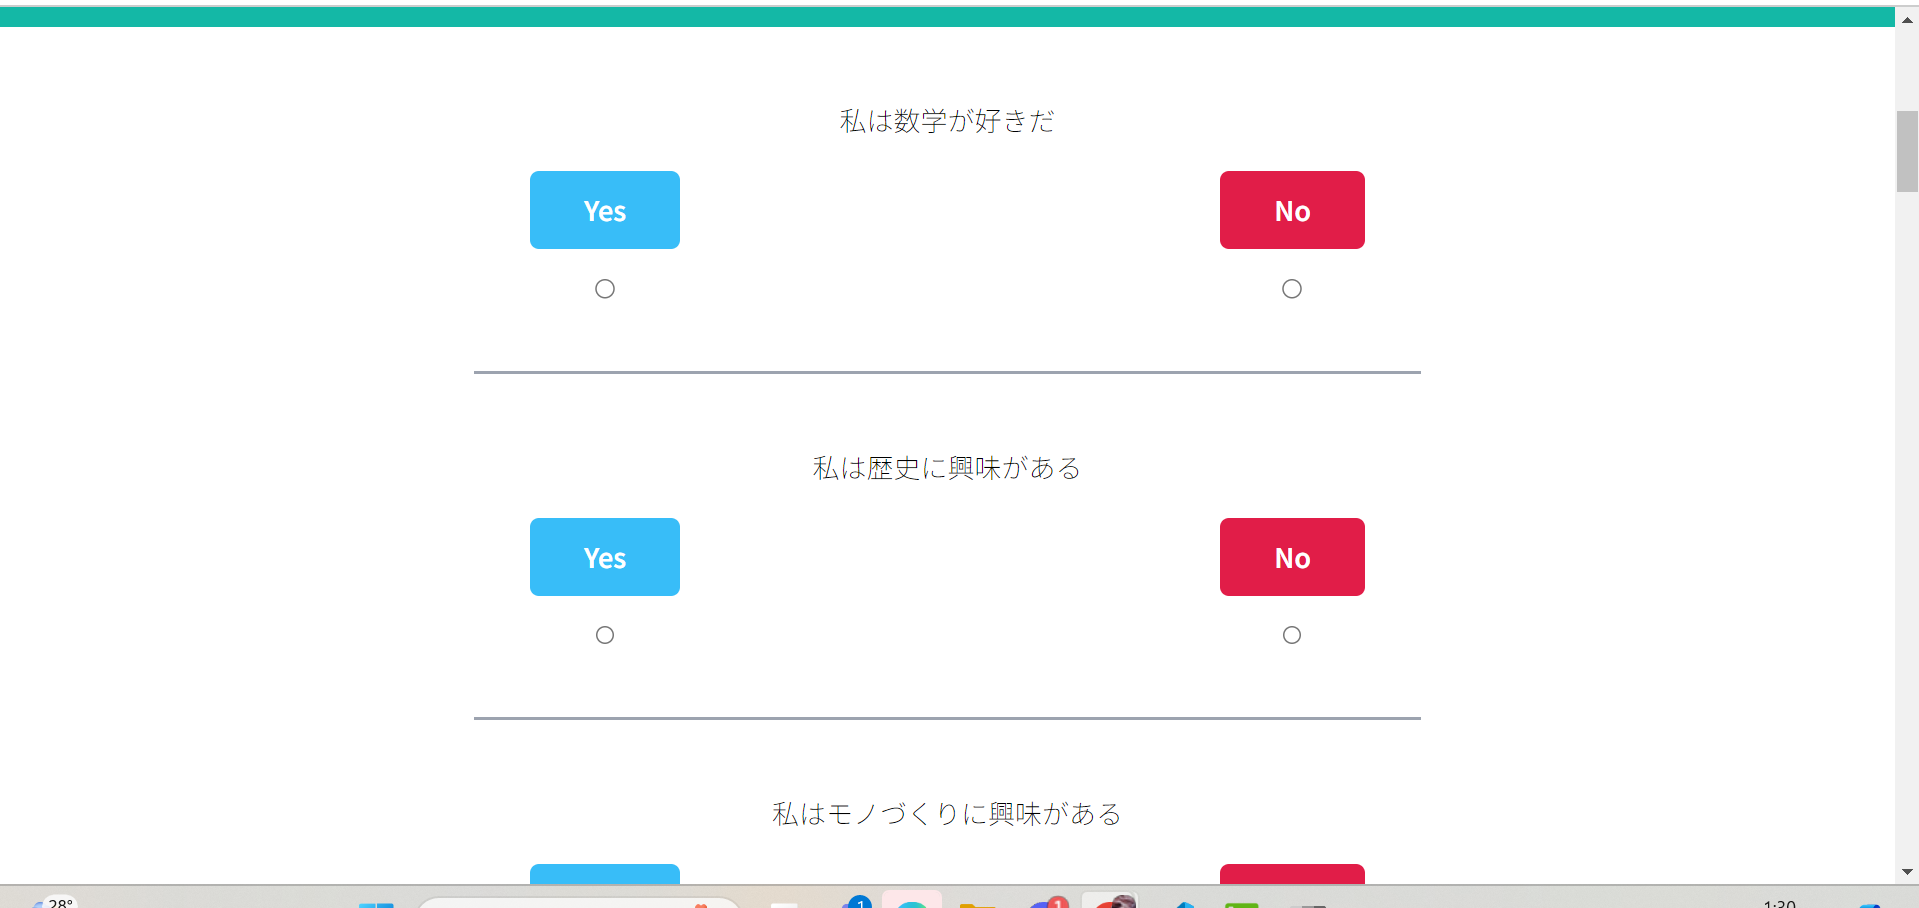
\includegraphics[width=100mm]{form2.png}
  \caption{フォーム}
  \end{center}
\end{figure}
\begin{figure}[htbp]
  \begin{center}
  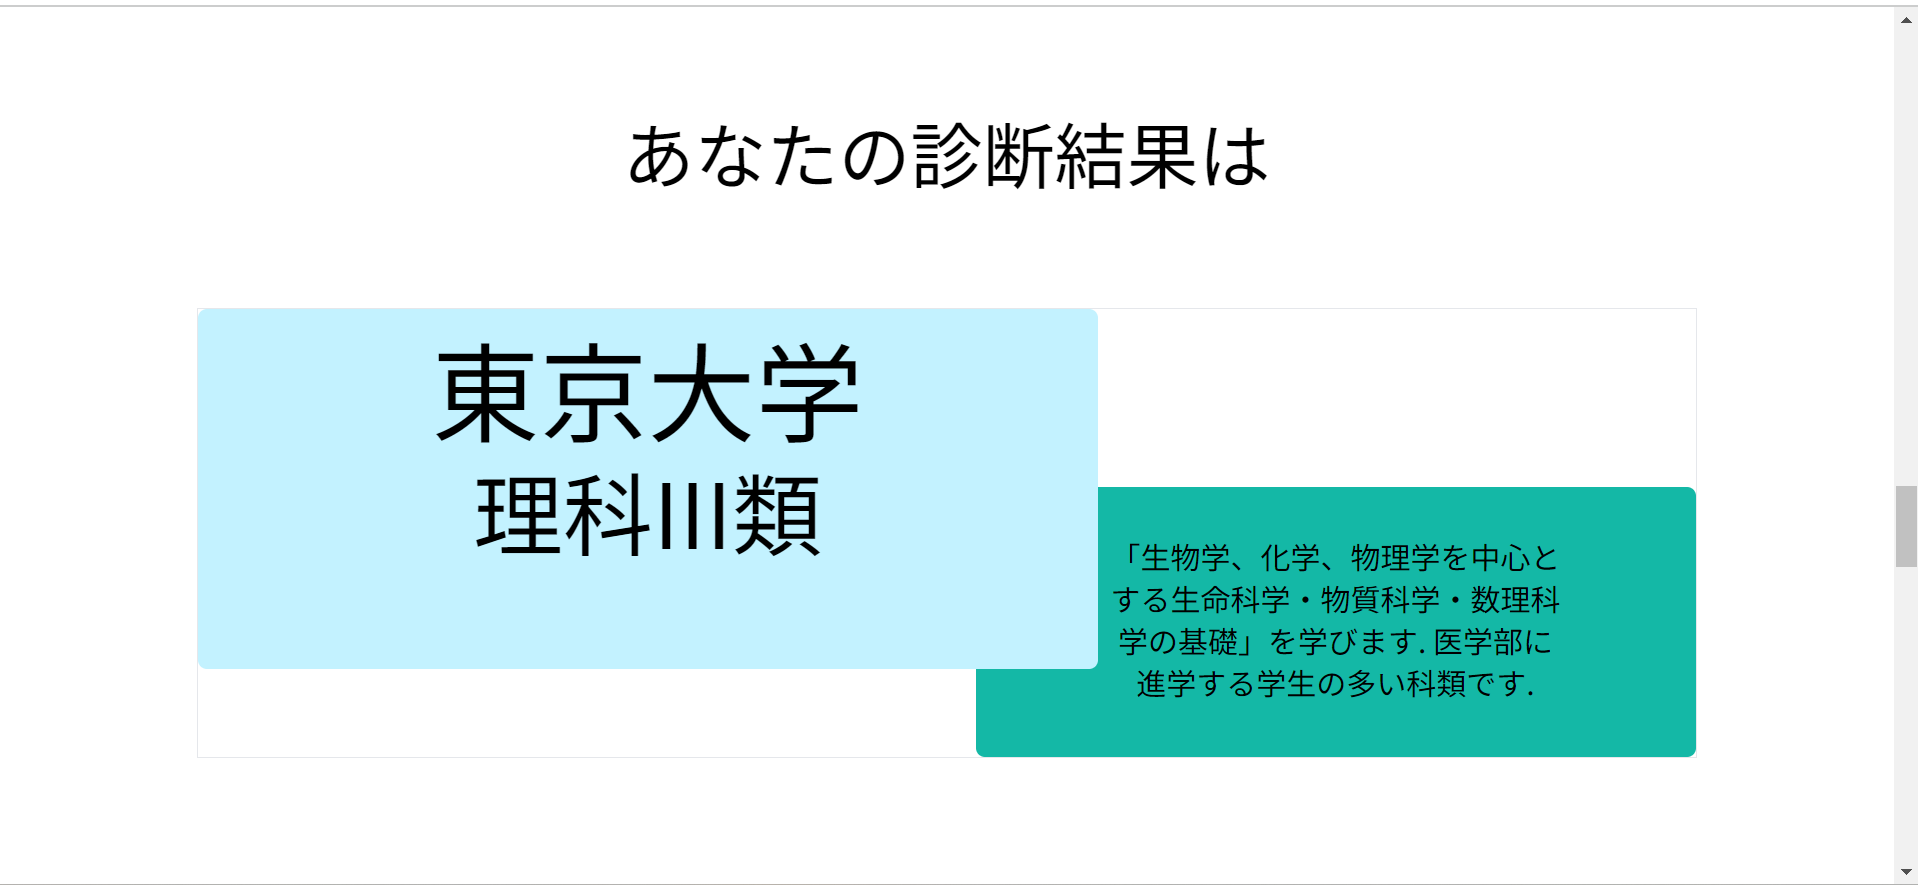
\includegraphics[width=100mm]{univs2.png}
  \caption{希望に沿った大学群}
  \end{center}
\end{figure}
\section{発表会終了時点でのTODOリスト}
以下,○を未完了事項,●を完了事項とする.\\
\\
●進路指導に必要なパラメータを考える\\
\\
●質問1つからなる簡単な進路指導システムの完成\\
\\
○生徒の偏差値帯を考慮したアプリケーションの作成\\
\\
○質問に対して正確に答えられていない場合のエラー出力の実装\\

\section{感想・謝辞}
本授業の遂行にあたり,大阪大学 大学院 情報科学科 松下 誠准教授にはレポートの書き方,効率的なチーム開発の方法等多岐に渡る指導を頂きました.また他の先生方にも議事録を通してのフィードバックや的確なアドバイスを頂き大変勉強になりました.ありがとうございました.
%\begin{thebibliography}[99]
%\item{}
%\end{thebibliography}

\end{document}
